% 第3章 HybriChain 系统设计

\chapter{HybriChain 系统设计}
\label{chap:design}

\section{问题定义与研究目标}

\subsection{核心问题}

在多语言混合编程的推理引擎中，安全分析人员面临一个根本性困境：推理引擎的语义边界（API 请求）与系统执行边界（内核 syscall/用户态函数）之间存在巨大的观测盲区。安全分析人员通过 HTTP 接口能拿到请求的输入与输出，但面对内部执行过程却无从下手：

\begin{itemize}
    \item 该请求在推理引擎内部触发了哪些函数调用？这些函数分别属于哪一层语言（Go、C、C++）？
    \item 推理引擎在内核层面进行了哪些系统调用？这些系统调用与推理计算的哪个阶段相对应？
    \item 若推理过程中出现异常（如内存分配失败、文件访问错误），该异常的根源在于哪一层代码？
\end{itemize}

推理引擎缺少跨语言调用链的有效观测工具。要做到这一点，需要回答一个关键问题——\textbf{如何在保证观测覆盖完备性的同时，将运行时开销控制在可接受范围内？}

具体而言，需要依次攻克以下三个子问题：

\begin{enumerate}[(1)]
    \item \textbf{高效且完备的函数调用追踪。} 原始函数调用数据是一切分析的前提。问题在于，推理引擎每秒产生数万次调用事件，全量追踪会让存储和计算资源迅速耗尽。追踪方案必须在覆盖范围与性能损耗之间找到平衡点。
    \item \textbf{高效统一的调用链合成与降噪。} 原始数据来自异构数据源（用户态函数调用、内核态系统调用），格式不统一、时间尺度不一致，大量与推理无关的噪声事件夹杂其中。必须先做降噪与合成，才能提取出可用的调用链。
    \item \textbf{准确的跨语言符号映射。} 合成后的调用链中，每条边对应一个函数符号（如 \texttt{compute\_forward}），但这些符号来自完全不同的命名空间——高层语言运行时、CGO ABI、底层计算库符号规范。缺少跨语言符号映射，就无法理解调用链从哪一层跨越到了哪一层。
\end{enumerate}

这三个子问题环环相扣：追踪提供原始数据，降噪合成让数据可用，符号映射让结果可解释。三者缺一不可。

\subsection{系统目标}

基于上述问题，本研究设计并实现了 HybriChain（Hybrid Engine Cross-Language Chain Analysis），一个面向多语言推理引擎的跨语言调用链追踪与安全分析系统，其设计目标如下：

\begin{enumerate}[(1)]
    \item \textbf{跨语言符号映射。} 将推理引擎内部来自不同编程语言（Go、C、C++）的函数符号统一映射到同一语义空间，构建跨语言全局调用图。
    \item \textbf{内核级运行时追踪。} 利用 eBPF 在零侵入的前提下，对推理引擎进行运行时函数与系统调用的双层观测，生成包含语义信息的调用事件流。
    \item \textbf{统一调用链缝合。} 将用户态函数调用与内核态系统调用按照时间顺序缝合为统一序列，形成端到端的推理调用链。
    \item \textbf{高效数据降噪。} 在数据采集端实施漏斗式降噪策略，将原始海量事件流压缩至可分析规模，释放后续图谱缝合引擎的内存与计算压力。
    \item \textbf{异常行为分析。} 在缝合后的调用链上实施规则驱动的异常检测，发现推理引擎中的潜在安全风险。
\end{enumerate}

\section{系统总体架构}

图~\ref{fig:system-arch} 给出了 HybriChain 的系统总体架构。系统部署于用户空间（Ring 3）与内核空间（Ring 0）两层，由被观测靶点（AI 推理引擎）与 HybriChain 分析系统两大部分构成，数据流向如下：

\begin{enumerate}[(1)]
    \item 用户端通过 HTTP 请求到达 API 前端，API 前端接收并转发请求；
    \item API 前端向推理执行器发起内部调用（IPC），触发跨语言调用链；
    \item 推理执行器发起系统调用（syscall），进入操作系统内核；
    \item 同时，静态符号提取模块通过解析推理引擎二进制文件，完成离线拓扑提取；
    \item eBPF 内核追踪模块在内核空间实时捕获系统调用事件流；
    \item 静态拓扑与动态轨迹汇聚至缝合与分析引擎，融合为统一调用序列；
    \item 缝合与分析引擎输出调用链图谱与异常告警，最终随推理响应一并返回用户。
\end{enumerate}

\begin{figure}[H]
    \centering
    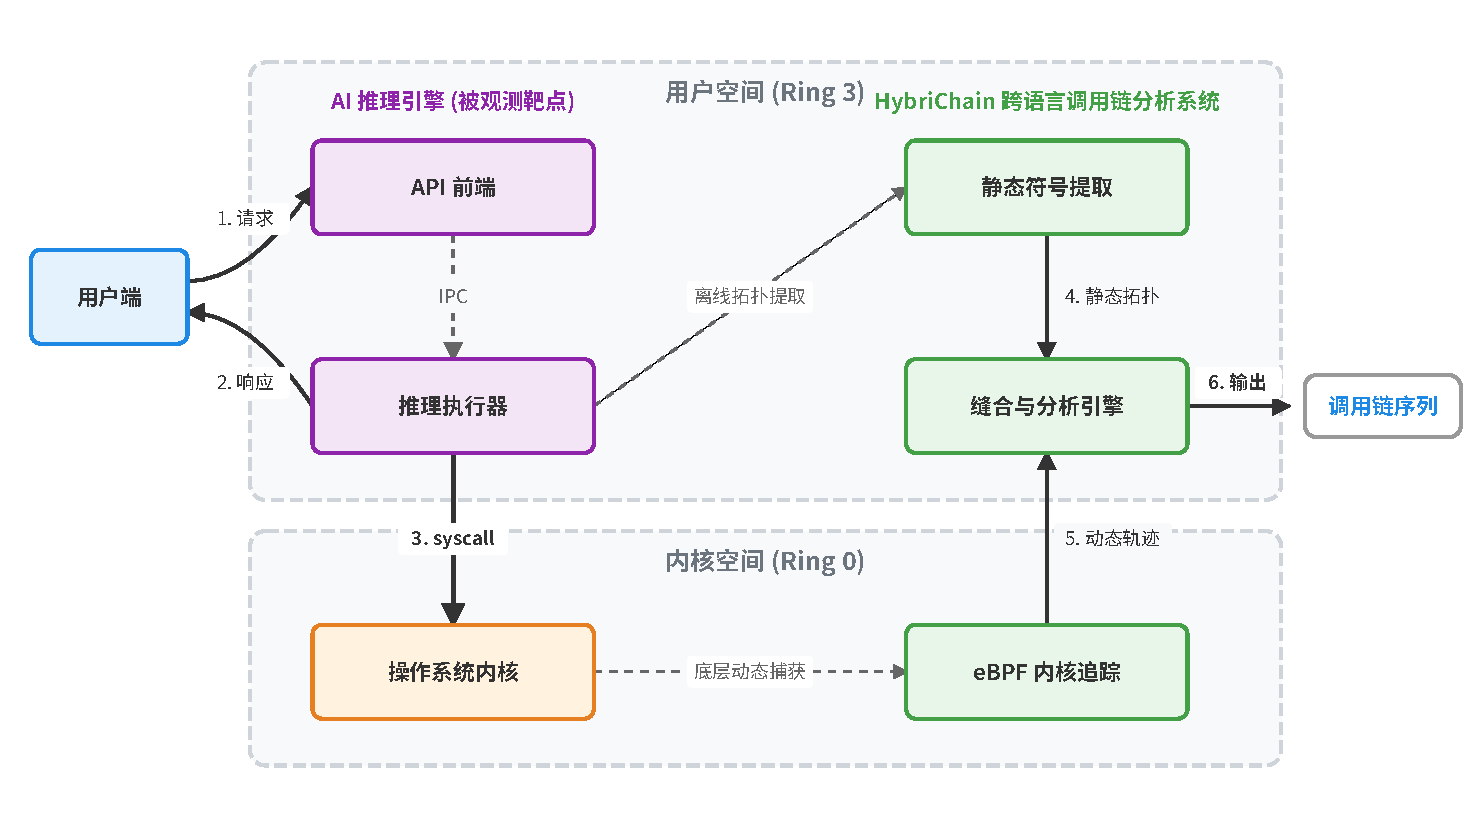
\includegraphics[width=0.90\textwidth]{figures/fig_architecture.pdf}
    \caption{HybriChain 系统总体架构}
    \label{fig:system-arch}
\end{figure}

HybriChain 分析系统内部包含三个核心模块：

\begin{itemize}
    \item \textbf{静态符号提取模块}（右中上绿色框）：在离线状态下对推理引擎二进制文件进行静态分析，提取各层（C/C++/Go）函数符号，构建跨语言调用图的节点集，覆盖全面但不含时序关系。
    \item \textbf{eBPF 内核追踪模块}（右中下绿色框）：以 eBPF 技术为核心，在内核空间实时捕获系统调用事件流，提供运行时真实数据但不含高层语义关联。
    \item \textbf{缝合与分析引擎模块}（右中中间绿色框）：将静态拓扑与动态轨迹融合，按时间戳对齐拼接统一调用序列，并在其上执行异常检测规则，输出带有置信状态的调用链图谱与风险告警。
\end{itemize}

\section{高效且完备的函数调用追踪}

上一节指出，为了获得跨语言调用链，第一个必须解决的问题是\textbf{高效且完备的函数调用追踪}——追踪提供原始数据，没有它后续一切无从谈起。但追踪必须满足两个要求：\textbf{完备性}（不能遗漏关键的跨语言边界节点）和\textbf{高效性}（不能对推理引擎造成不可接受的性能退化）。

追踪的困难主要来自推理引擎函数调用的固有特点：每秒可产生数万次函数调用和系统调用；调用栈深度可达数十层，跨越多层编程语言（如 Go 运行时、CGO 桥接层、底层计算库等）多个语义层次；若不加选择地追踪所有函数，数据量将以不可承受的速度增长。

因此，HybriChain 采用\textbf{探针下沉策略}（Probe Sinking Strategy），将追踪点精确下沉至推理引擎的三个关键层次：

\begin{enumerate}[(1)]
    \item \textbf{推理计算函数层（用户态 uprobe）}：在推理引擎的核心函数上附加 uprobe，如张量计算入口、采样入口、同步点等。该层提供推理过程的微秒级耗时数据，是跨语言调用的直接证据。
    \item \textbf{系统调用层（内核 tracepoint）}：在内核系统调用入口与返回点附加 tracepoint，记录推理引擎向内核发起的全部系统交互（read/write/futex/mmap/clone3 等）。该层提供毫秒级时间精度，反映推理引擎与操作系统之间的资源交互行为。
    \item \textbf{内存分配层（内核 mmap tracepoint）}：专门追踪 mmap/munmap 系统调用，提取内存分配大小与地址信息，用于分析推理引擎的缓存分配行为——这是推理引擎内存消耗的主要来源。
\end{enumerate}

eBPF 相比传统追踪工具（strace、DTrace），在内核中运行，无需修改目标程序代码，具备即时生效的热更新能力，且通过 RingBuf 实现零拷贝数据传输，将追踪对推理性能的影响降至最低。

在探针附加策略上，本系统采用"保守挂载 + 增量采集"原则：\textbf{仅对推理计算相关函数挂载 uprobe}，而非追踪所有函数，从而将运行时开销控制在可接受范围内。

\section{高效统一的调用链合成与降噪}

有了原始的追踪数据，第二个必须解决的问题是\textbf{高效统一的调用链合成与降噪}——原始数据来自多个异构数据源，数据格式不统一，且充斥着大量与推理无关的噪声事件，不经过处理无法形成可用的调用链。

降噪的必要性在于，推理引擎在内核层面每秒可产生数万条系统调用事件，其中大量是与推理计算无关的噪声事件，例如：频繁的 \texttt{brk} 调用（堆内存微调）、\texttt{mprotect} 保护调整调用、读取 \texttt{/dev/zero} 和 \texttt{/dev/urandom} 等设备文件。若将原始事件流全部存储，不仅存储成本爆炸式增长，后续缝合引擎也将在海量噪声数据中迷失方向。

HybriChain 设计了\textbf{漏斗式降噪流水线}（Noise Reduction Pipeline），将原始内核事件流逐步压缩至仅包含强语义节点的事件集。具体处理步骤如下：

\textbf{步骤一：元信息过滤。} bpftrace 的文本输出包含大量元信息行（如 "Tracing... Stop: Ctrl+C ..." 等），直接过滤。

\textbf{步骤二：进程过滤。} 仅保留推理引擎相关进程的系统调用，排除其他进程的干扰。

\textbf{步骤三：类型过滤。} 对系统调用类型进行白名单过滤——仅保留高频语义事件（read/write/mmap/futex/clone3/openat），过滤掉 brk/mprotect/madvise/munmap 等高频内存调整调用。

\textbf{步骤四：参数过滤。} 对保留的系统调用进行参数级过滤——例如，read 调用仅记录有效文件描述符（fd $\geq$ 3）且字节数 $> 0$ 的事件，排除读取 /dev/zero 等噪声操作；mmap 调用仅记录分配大小 $\geq$ 1MB 的事件，排除微小的堆扩展请求。

\textbf{步骤五：栈帧清洗。} 对 uprobe 收集的调用栈进行符号化处理，过滤内存地址（0x 开头），仅保留可读的函数符号名，并进行 C++ demangle 处理。

经过上述五步漏斗降噪，原始事件流的数据量通常压缩 2–3 个数量级，为后续图谱缝合引擎释放了可观的内存与计算资源。

\textbf{为什么缝合是必需的？} 降噪后的数据仍然是两类分散的事件集合——uprobe 事件（用户态函数调用）和 tracepoint 事件（内核态系统调用）。两者处于不同的抽象层次，时间精度也不一致（微秒 vs 毫秒），无法直接拼接成一条完整的调用链。因此，需要按时间戳顺序将两类事件缝合为统一序列，并在缝合过程中为每条跨语言边赋予置信状态。

HybriChain 采用基于时间戳对齐的启发式缝合算法，按以下策略赋予置信度：

\begin{enumerate}[(1)]
    \item \textbf{Confirmed（确认）}：通过调用栈上下文直接确认的跨语言调用关系，如 uprobe 中调用栈明确包含 CGO 桥接函数，表明上一层直接调用了下一层；
    \item \textbf{Inferred（推断）}：通过时间窗口启发式推断的调用关系，如 \texttt{mmap} 系统调用在某次推理函数调用之前某个时间窗口内触发，且内存大小符合推理引擎缓存分配特征（数百 MB）；
    \item \textbf{Conflicting（冲突）}：同一对节点存在多个时间窗口相互矛盾的推断，说明该边可能不稳定；
    \item \textbf{Unknown（未知）}：静态符号存在于调用图中，但动态追踪未观测到实际调用关系，说明该路径未被触发。
\end{enumerate}

\textbf{为什么需要置信度？} 因为跨语言边界上的调用关系无法通过单一数据源完全确认。调用栈可以确认有直接调用关系（Confirmed），但大量的系统调用只能通过时间窗口推断（Inferred）。置信度让分析人员能够区分哪些调用关系是确定的，哪些是推测的，从而做出可靠的安全判断。

缝合的输出为：按时间排序的统一调用序列，每条事件携带类型（uprobe/syscall）、所属推理阶段、风险等级与置信状态等元信息。

\section{准确的跨语言符号映射}

有了可用的缝合调用链，第三个必须解决的问题是\textbf{准确的跨语言符号映射}——缝合出的调用链中每条边代表的是函数符号，但这些符号来自完全不同的命名空间，若不建立映射关系，分析人员仍然无法理解一条调用链从哪一层跨越到哪一层。

\textbf{为什么符号映射如此困难？} 推理引擎的函数符号来自三个完全不同的命名空间：高层语言运行时符号（如 goroutine 调度器、网络/文件接口）、语言桥接层导出符号（CGO 桥接函数、Python C Extension 等）、底层计算库符号（如神经网络算子库，遵循各语言自己的符号规范）。三者的命名规则完全不同，直接拼接会导致符号空间割裂——高层语言侧的符号无法与底层库侧的符号建立语义关联。

HybriChain 提出一种\textbf{五层符号分类体系}，按语义层次对推理引擎内部函数进行统一分类。表~\ref{tab:layer_classification} 给出了该分类体系的具体定义。

\begin{table}[H]
    \centering
    \caption{五层符号分类体系}
    \label{tab:layer_classification}
    \begin{tabular}{|c|c|p{7.5cm}|}
        \hline
        \textbf{层次} & \textbf{名称} & \textbf{说明} \\
        \hline
        f\textsubscript{0} & 系统边界层（System Boundary） & 负责与操作系统交互的函数，包括文件 I/O（open/read/write/close）、内存管理（mmap/brk/mprotect）、进程管理（clone/execve）等。该层函数命名遵循 POSIX 标准，与语言无关 \\
        \hline
        f\textsubscript{1} & 运行时胶水层（Runtime Glue） & 负责语言间调用的桥接函数，在 CGO 体系中表现为以 \texttt{cgo:} 为前缀的包装函数，在 Python C Extension 中表现为 \texttt{PyCFunction} 类型的导出函数，是跨语言调用的关键节点 \\
        \hline
        f\textsubscript{2} & 张量计算层（Computation） & 负责神经网络推理的核心计算函数，如矩阵乘法、注意力机制、激活函数等，通常以 CUDA kernel 或 CPU SIMD 实现，函数名具有领域特定模式（如 \texttt{matmul}、\texttt{attention}、\texttt{softmax}） \\
        \hline
        f\textsubscript{3} & 内存管理层（Memory） & 负责缓存分配与释放、模型权重加载、上下文管理的函数，该层调用频繁且与系统调用层（mmap）存在直接映射关系 \\
        \hline
        f\textsubscript{4} & 调度协调层（Scheduling） & 负责任务分发、线程池管理、锁与同步操作的函数，通常表现为高频的 futex 系统调用，是推理引擎并发性能的瓶颈所在 \\
        \hline
    \end{tabular}
\end{table}

\textbf{五层分类如何支撑准确的符号映射？} 每一层（f$_0$–f$_4$）对应推理引擎中一类明确的语义角色。给定任意一个函数符号，通过关键词匹配和命名规范分析即可确定其所属层次。例如，以领域特定前缀（如 \texttt{tensor\_}、\texttt{matmul\_}）命名的函数属于张量计算层（f$_2$），以 \texttt{cgo:} 为前缀的函数属于运行时胶水层（f$_1$）。由此，任意两个跨层调用（如 f$_1$ $\to$ f$_2$）都有了语义上的解释：

\begin{itemize}
    \item f$_1$（胶水层）$\to$ f$_2$（计算层）：高层语言层通过语言桥接调用了底层计算库的推理函数
    \item f$_2$（计算层）$\to$ f$_0$（系统层）：推理计算触发了 mmap 内存分配
    \item f$_4$（调度层）$\to$ f$_0$（系统层）：调度线程发起了 futex 同步操作
\end{itemize}

五层分类体系为每一条缝合出的调用链边赋予了跨语言的语义身份，使原本割裂的多语言符号空间统一到同一语义坐标体系中。

\section{异常检测规则引擎设计}

在缝合后的统一调用序列（§3.4）与五层符号分类体系（§3.5）的基础上，HybriChain 通过规则引擎对推理引擎运行时行为进行异常检测。

规则引擎的工作流程分为三步。首先遍历每条调用事件，根据事件类型（uprobe/syscall）、函数名、时间戳等字段做模式匹配。匹配成功后进入判断阶段，检查系统调用耗时是否超过阈值、文件路径是否落在敏感目录、内存分配大小是否偏离正常范围。条件成立时即生成结构化告警，包含时间戳、线程ID、告警类型、风险等级（LOW/MEDIUM/HIGH）及详细上下文。

每条规则独立运行，互不干扰，最终告警按风险等级聚合输出。

\section{本章小结}

本章阐述了 HybriChain 的系统架构与核心设计。各模块的设计动机可以归纳为一条主线：

\begin{itemize}
    \item 获取跨语言调用链的前提是高效且完备函数调用追踪（§3.3），为此设计了探针下沉策略，将追踪点精确放置在推理计算函数层、系统调用层和内存分配层三个关键位置；
    \item 原始追踪数据无法直接使用，需要进行调用链合成与降噪（§3.4），具体实现为五步漏斗式数据降噪流水线和基于时间戳对齐的跨语言缝合算法，缝合结果为每条边标注置信状态；
    \item 缝合出的调用链要让人看懂，需要跨语言符号映射（§3.5），由此提出五层符号分类体系（f$_0$–f$_4$），把不同命名空间的函数符号映射到同一语义坐标中；
    \item 在以上成果的基础上，异常检测规则引擎（§3.6）在缝合后的调用链上执行规则驱动的异常检测。
\end{itemize}

下一章将以 Ollama 推理引擎为具体靶点，逐一展开各设计方案在工程实践中的实现细节。
